%%%%%%%%%%%%%%%%%%%%%%%%%%%%%%%%%%%%%%%%%%%%%%%%%%%%%%%%%%%%%%%%%%
\section{Existing Calibration Sources} \label{sec:existsource}

All dedicated external calibration systems must provide benefits outside of free, copious, and commonly used calibration sources, described in this section. DUNE will use particles from cosmic ray muons (Section~\ref{sec:cr}), neutrino-induced interactions (Section~\ref{sec:nuinduced}),  argon isotopes (Section~\ref{sec:ar39}) and information from instrumentation data  (Section~\ref{sec:inst}). Cosmic rays and neutrino-induced interactions provide commonly used ``standard candles'' like electrons from muon and pion decay, and neutral pions, which have characteristic energy spectrums. 

%%%%%%%%%%%%%%%%%%%%%%%%%%%%%%%%%
\subsection{Cosmic Rays }\label{sec:cr}
%- Tom Junk first draft}

Cosmic-ray events will provide the second-largest source of ionization charge in the DUNE \dword{fd},
after radiological decays.  Depending on the triggering strategy, cosmic-ray events may contribute the
most to the data volume from the \fardet.  Starting from a predicted rate of four cosmic-ray muons
per square meter per day at the 4850' level at SURF~\cite{LBNEDOCDB9673}, we expect 
approximately \num{3}~million cosmic-ray particles per year for the four-module \dword{fd}.
A sample of \num{20000} cosmic-ray muons was simulated for a % single-phase 10~kt module 
\SI{10}{\kt} \dword{spmod} using the MUSUN
generator~\cite{Kudryavtsev:2008qh} and reconstructed using \dword{larsoft}.  This simulation draws muon
momenta from a pre-computed spectra with full angular and energy dependence given the local rock
composition and topography at the SURF laboratory.  The energy and angular distributions are given
in~\cite{LBNEDOCDB9673}.  The MUSUN generator only simulates single cosmic-ray muons;
muon bundles arising from high-energy atmospheric showers are not simulated yet.
The rates are uncertain at the level of 20\%.

Cosmic rays can provide many critical measurements for DUNE, described in the following subsections. These include detector timing offsets, detector alignment, drift velocity, electron lifetime, relative channel calibrations, absolute gain,  electromagnetic response using decay electrons and $\pi^0$.
%These cosmic-ray events can be used to calibrate detector element locations, as well as the response of the detector to high-energy particles. 
Some events may be useful for some measurements and not others.  For example, detector alignment studies require muons that pass over the gaps between
\dwords{apa}, or pierce the \dwords{apa} or  \dwords{cpa}, while studying the electron drift and lifetime requires muons
that traverse the entire horizontal drift direction between the \dwords{apa} and \dwords{cpa}.  In the list of
possible measurements below, we estimate the daily rate of cosmic-ray muon events that can be used
and the requirements used to select these events.

%\subsubsection{Possible Measurements}
%%%%%%%%%%%%%%%
\subsubsection{Detector Timing Offsets}

A measurement of the global time offsets between the TPC wire readout and the photon detectors
and external sources of timing information (such as external muon counters), can be made
with tracks that cross through the \dword{apa} volumes.  Hits on either side of the \dwords{apa} drift in opposite
directions and thus a constrained fit for a track to line up on both sides of an \dword{apa} requires the
time of the event to be correct.  Hits that drift from locations close to the \dwords{apa} are minimally
affected by space charge and other field distortions.

Approximately six non-showering muons are estimated to pierce each \dword{apa} per day.  This number
is the nine muons per day crossing a vertical gap, which is estimated in the next section, multiplied
by (\SI{2.5}{\m})/(\SI{3.6}{\m}), the ratio of the width of an \dword{apa} to the drift distance.  Timing offsets can therefore
be measured in under a week on an \dword{apa} by \dword{apa} basis, and a global timing offset with less than a day's worth
of data.
 
 %%%%%%%%%%%%%%%%%
\subsubsection{Detector Alignment}

The 150 \dwords{apa} in a \dword{spmod} are expected to be rigid bodies that are assembled to
precise mechanical tolerances.  The requirements for physics analyses however often exceed 
mechanical tolerances that can be achieved, especially after cool down.  Straight tracks that cross
from the volume of liquid argon that is read out by one \dword{apa} into the volume read out by another \dword{apa}
give, by steps in their apparent positions and angles, constraints on the relative positions and angles
of the \dwords{apa} as they are situated in the detector.   A full alignment campaign using cosmic rays will
find the minimum of a $\chi^2$ function that depends on the measured track segments, positions and angles of
the \dwords{apa} and  \dword{cpa} panels, and includes any external constraints such as mechanical surveys, along with
realistic uncertainties.  Examples of cosmic-ray alignment campaigns can be found from 
ATLAS~\cite{LacuestaMiquel:2015ksh,Moles-Valls:2014wza}, CMS~\cite{Chatrchyan:2009km}, ALICE~\cite{Aamodt:2010aa}.
In the following discussion, the $y$ axis is vertical, the $x$ axis points along the electric field,
and $z$ points approximately along the beam direction.

Given experience from the \dword{35t}, we predict
that the precision on the width of a vertical gap between two neighboring \dwords{apa} is
\begin{equation}
\sigma_{\Delta z} \approx \frac{1.79\times 10^{-1}~{\rm{cm}}}{\sqrt{N_{\rm{tracks}}}},
\end{equation}
where $N_{\rm{tracks}}$ is the number of cosmic-ray muon tracks used to make the measurement,
and the precision on offsets in the \dword{apa} positions along the drift direction (aplanar steps) is
\begin{equation}
\sigma_{\Delta x} \approx \frac{5.83\times 10^{-2}~{\rm{cm}}}{\sqrt{N_{\rm{tracks}}}}.
\end{equation}
Naively taking the top half of an \dword{apa} as a separate measurement from the bottom half and using these
precisions to estimate angular resolutions.  We thus estimate
\begin{equation}
\sigma\left(\frac{d\Delta z}{dy}\right) \approx \frac{\sqrt{2}\sigma_{\Delta z}(N_{\rm{tracks}}/2)}{3~{\rm{m}}}
\approx
\frac{1.19\times 10^{-3}}{\sqrt{N_{\rm{tracks}}}}
\end{equation}
and
\begin{equation}
\sigma\left(\frac{d\Delta x}{dy}\right) \approx \frac{\sqrt{2}\sigma_{\Delta x}(N_{\rm{tracks}}/2)}{3~{\rm{m}}}
\approx
\frac{3.89\times 10^{-4}}{\sqrt{N_{\rm{tracks}}}}.
\end{equation}


The numbers of tracks available to make these measurements depends on the energies, positions, and angles
required.  The energy of muons is required to be less than \SI{485}{\GeV}, the critical energy in \dword{lar},
above which bremsstrahlung and pair production dominate the energy losses over ionization.  Tracks
that have too many electromagnetic showers along their lengths cannot be used for alignment, though
analyses that use track sections that are locally straight might be able to recover a fraction of these.
We require that at least \num{20} collection-plane wires are hit by a track on either side of a vertical gap, providing
enough space points to measure the parts of the track on either side of the gap.  Saturation of the \dword{adc}
is an issue for some measurements but should affect alignment studies less than lifetime and signal
strength calibrations, so the geometrical requirement is currently estimated to be sufficient.
Given the full simulation and these requirements, approximately nine muons that can be used for alignment
pass through the argon over a vertical gap every day.  Horizontal gaps between \dwords{apa} that are stacked
vertically are shorter, but given the dominantly vertical direction of the incident muons are easier
to hit per unit area.  We estimate that ten muons per day pass through a horizontal gap and can be
used for alignment.

The cathode planes provide additional alignment tasks that can be addressed with cosmic rays.
Because there are six cathode plane panels per \dword{apa}, there are more alignment parameters to consider.
Similarly to the ICARUS experience, the volume on both sides of the cathode planes is active, and charge
drifts in opposite directions on the sides of the cathode.  Thus, if a cathode plane element is displaced
in $x$, a track that pierces it will appear to extend beyond the physical location.  We assume the
same rate of cosmic-ray muons piercing the cathode planes per unit area as for the \dword{apa} planes, which
means one muon per day per cathode-plane panel is expected.  A full alignment with \SI{1}{\m$^2$} pixels of the
ICARUS cathode took roughly six months of data, and it is reasonable to expect a similar amount of time
needed to fully align the cathode panels of DUNE.

One of the main drivers of precise alignment is to be able to use multiple scattering in order to
measure muon momentum for muons that escape the detector before stopping.  
This analysis has been performed by ICARUS~\cite{Antonello:2016niy} and by \microboone~\cite{Abratenko:2017nki}.
Residual uncertainties in the cathode plane flatness in were the limiting systematic uncertainties
in the ICARUS measurement.

%%%%%%%%%%%%%%%%
\subsubsection{Drift Velocity and TPC Size}

Tracks that pierce both an anode plane and a cathode plane in DUNE are particularly valuable. %because
The difference in arrival times of the drifting charge gives the total drift distance divided by the
drift velocity, assuming one of these quantities gives a measurement of the other.

%%%%%%%%%%%%%%%%
\subsubsection{Electron Lifetime}

Tracks that leave ionization at a variety of different distances from the anode provide a sample
with which to measure the electron lifetime.  Two similar methods have been used.  In the
first, track charge deposits $dQ/dx$ are measured, the highest and the lowest are ignored because
the tail of the Landau offers less information than the core, and an exponential is fit on a 
track-by-track basis.  The track-by-track electron lifetime is then averaged over many such tracks
(the reciprocals are in fact averaged to help remove biases due to asymmetric uncertainties).  In
the second method, a single exponential is fit to the sum of the measured $dQ/dx$ values for many tracks.
Examples of these methods can be found from ICARUS~\cite{Antonello:2014eha}, 
\microboone~\cite{MICROBOONE-NOTE-1026-PUB}, as well as in the \dword{35t} and
the LArIAT detectors\fixme{references for 35t is "M. Thiesse, Ph.D. Thesis, University of Sheffield, 2018)" and LArIAT?}.  Extrapolating from the ICARUS precision on $\lambda = 1/\tau$, we expect
that each cathode-anode piercing track will provide a $\pm 30$\% measurement of the lifetime
at a lifetime of \SI{3}{\milli\s}.

If one requires tracks to pierce both an anode plane and a cathode plane and have an energy between \SI{20}{\GeV}
and \SI{400}{\GeV} in order to be straight and non-showering, then the rate is five per day per drift volume
on one side of an \dword{apa}.  If one further requires that the muon pierce one of the six cathode panels
directly opposite to the \dword{apa} it pierced, then the rate falls to \num{1} per day.  \dword{adc} saturation is not
a concern for tracks that traverse the entire drift length.

%%%%%%%%%%%%%%%%
\subsubsection{Relative Channel Calibration}

Channel-to-channel gain variations can be tested with large samples of cosmic-ray muons.  The rate at
which a single collection-plane channel records useful data from cosmic-ray muons is very similar to that
for the vertical gaps between \dwords{apa}, or roughly ten per day.  In this case, \dword{adc} saturation is a concern,
but traversing forty collection-plane wires in the \SI{6}{\m} height as per the angular requirement for alignment
should keep the hits from saturating the \dwords{adc}.

Nonetheless, a comparison of the gains of faraway channels requires averaging over a large ensemble
of cosmic-ray muons, as the muons will have different energies and thus different $dE/dx$ values,
and given their dominant vertical directions, each will hit only a portion of an \dword{apa}.  A high-precision
calibration of each channel's relative gain will likely take on the order of months, depending
on the track-to-track variation in measured $dQ/dx$ values which affects the rate of convergence
of the average.

%%%%%%%%%%%%%%%%
\subsubsection{Absolute Gain Calibration with Minimum Ionizing Particles}

A measurement of the Minimum Ionizing Particle (MIP) scale in the DUNE \dword{fd} will be more challenging, as the $dE/dx$
distribution depends on the energies of the incident muons.  With a model of the energies,
one can find the distribution of $dQ/dx$ values and fit it with a floating global gain value
and uncertainties in the parent energy distribution to obtain a global scale. This method
is subject to systematic uncertainties arising from the energy scale of the incident muons.

%%%%%%%%%%%%%%%%
\subsubsection{Electron Response Calibration from Michel Electrons}

Stopping $\mu^+$ particles will produce Michel electrons with a known energy spectrum which can
be used to calibrate the response of the detector.  An example analysis of Michel electron
reconstruction is available from \microboone~\cite{Acciarri:2017sjy}.  This analysis is sensitive
to the collection of energy deposited by bremsstrahlung photons which Compton-scatter a short distance away from
the Michel electron, and is useful in tuning up reconstruction as well as the simulation.  Approximately
\num{30} muons per day are expected to stop in a \SI{10}{\kt} module.

%%%%%%%%%%%%%%%%
\subsubsection{Electromagnetic Energy Scale from $\pi^0$ Decays}

An estimate of the rate at which cosmic-ray muons produce $\pi^0$s is of the order of one per \num{1000}
cosmic rays.  The ICARUS experiment performed an analysis of \num{212} candidate $\pi^0$ decays
from the 2001 Pavia surface test run~\cite{Ankowski:2008aa}. 
%The rate is expected to be low in the far detector, and may be overshadowed by atmospheric neutrino interactions. %% KM our other table says 300 atm nu induced vs. 3000 here

% Table or text about rates of each category of event. 

%%%%%%%%%%%%%%%%
\subsubsection{Limitations}

As described in Refs.~\cite{LacuestaMiquel:2015ksh,Moles-Valls:2014wza}, alignment of detectors using
only cosmic-ray muons leaves some combinations of uncertain parameters only loosely constrained.
These are labeled ``weak'' directions in the citations above.  While the DUNE \fardet geometry is
significantly different from a collider detector, similar weak directions will appear in the cosmic-ray
alignment campaign.  Distortions of the detector that preserve the gap widths and do not shift
the \dwords{apa} in $x$ near the gaps relative to one another will be difficult to measure with cosmic rays.
These distortions include global shifts and rotations in the locations of all detector elements,
and crumpling modes where the edges of the \dwords{apa} hold together but angles are slightly different
from nominal.  An example of such a distortion is shown in Figure~\ref{fig:apacurtainalign}. 

\begin{dunefigure}[Sample distortion that may be difficult to detect with cosmic rays]{fig:apacurtainalign}{An example of a distortion that may be difficult to detect with cosmic rays.  The \dword{apa} frames are shown as
rotated rectangles, as viewed from the top.}

\includegraphics[width=0.8\textwidth]{apacurtainalign.png}
\end{dunefigure}

There is a global degeneracy between the drift velocity and the drift distance scale in the \dword{fd},
as measured with cosmic-ray muons.

The uncertainty in the energy spectrum of cosmic-ray muons is a limitation on the global \dword{mip}
calibration using these events.

Some of the measurements described above, such as the channel-to-channel gain uniformity and the
cathode panel alignment, are estimated to take months of data.  We will initially assume that
the calibration parameters are constant and average over the data as it comes in, and only after
larger data samples have been accumulated can more differential measurements be made, such as
constraining time dependence of channel gains and spatial dependence of the electron lifetime.

%%%%%%%%%%%%%%%%
\subsubsection{Remaining Studies}

Each of the analyses described here requires a full effort to carry to completion with data.
Estimates of sensitivity using simulated data can be used to estimate the levels of precision expected
as functions of time.  

The remaining studies for calibration for the TDR related to cosmic ray samples is:
\begin{itemize}
\item Quantify what can be achieved for  electron lifetime measurements and the overall energy scale calibration from cosmic rays in terms of spatial and temporal granularity.
\item Determine what weakly constrained misalignment modes may be important to understand for the physics case. It is expected that combinations of information from cosmic-ray events with other calibration sources (laser-based, neutrino-induced events, and dedicated muon systems) will reduce the total uncertainties, especially for alignment modes which are weakly constrained due to cosmic ray direction. 
\end{itemize}

%The impact on the physics of these weakly constrained modes needs to be determined to assess how critical the redundancy is.


%%%%%%%%%%%%%%%%%%%%%%%%%%%%%%%%
\subsection{Neutrino-induced interactions }\label{sec:nuinduced}
%- Vitaly draft; editing by Kendall}

%{\it stopping protons?} \\

Beam and atmospheric neutrinos and antineutrinos will provide interactions useful for certain calibrations of the \dword{fd}.%DUNE FD. 
Both sources of neutrinos will produce CC and NC events, where CC interactions will produce a muon or an electron in the event. Table \ref{table:nu-rates} summarizes event rates from different neutrino sources. Neutrinos (or antineutrinos) will produce muons outside and inside the detector that can be tagged as partly or fully contained events. Fully contained events provide more information since the total energy (and the total muon energy) can be reconstructed from the muon range and $dE/dx$. 

\begin{dunetable}[Atmospheric and beam neutrino and antineutrino event rates per year]{lc}{table:nu-rates}
{Atmospheric~\cite{Acciarri:2015uup} and beam neutrino and antineutrino event rates per year in \SI{40}{\kt} fiducial mass of the \dword{fd}. The beam-rock interaction rate is for the front (beam direction) face of the \dword{detmodule} %DUNE cryostat 
only; additional interactions will occur along the side.} % of the cryostat. }
%\begin{center}
%\begin{dunetabular}{|c|c|}
%\hline
\textbf{Event type} & \textbf{Rate/year/40 kt}\\ \hline
Fully contained atmospheric $e$-like & $1.6\times10^{3}$ \\ \colhline
Fully contained atmospheric $\mu$-like & $2.4\times10^{3}$ \\ \colhline
Partly contained atmospheric $\mu$-like & $7.9\times10^{2}$ \\ \colhline
CC or NC atmospheric $\pi^0$ & $300$ \\ \colhline
CC or NC atmospheric $K^+$ & $20$ \\ \colhline %(K+) is less than 1% of events (0.7-0.8%), so we may have 20 per year in 40 kt. This is from Andy’s Blake LBNE note 8836. KM couldn't find reference
Beam induced, rock\cite{bib:docdb6628} $\mu$-like & $2.8-5.6\times10^{3}$ \\ \colhline
Beam induced, \dword{lar} (signal) $\mu$-like & $2.8\times10^{3}$ \\
%\end{tabular}
%\end{center}
\end{dunetable}
 
 %%%%%%%%%%%%%%%%
 \subsubsection{Possible Measurements}
   
%Beam and atmospheric neutrinos will provide interactions useful for certain calibrations of the DUNE FD. Both sources of neutrinos will produce CC and NC events, where CC interactions will also provide a muon and electron in the event.
%with CC events resulting in better energy reconstruction of the whole event and in muons or electrons useful for calibrations. 

%However, the calibration use of some of the  the use of fully contained beam-Ar induced events must be treated with care as these events are  The use of beam-induced electron-like events is limited because they also represent signal events in the detector. 

%I think, the kaon production (K+) is happening in less than 1% of events (0.7-0.8%), so we may have 20 per year in 40 kt. This is from Andy’s Blake LBNE note 8836.

Although cosmic-ray muons have much higher event rates compared to atmospheric or beam neutrinos, CC events from neutrino interactions have a few advantages. Beam events will complement cosmic-ray muon calibration, in particular at near-horizontal directions ($\cos\theta < 0.3$) where cosmic-ray muons are absent. Neutrino-induced muons will help with testing the \dword{apa} alignment. However, only muons with relatively high energy will provide accurate measurements since low-energy muons may undergo multiple coulomb scattering.

Both partially and fully contained muon events will provide a sample of electrons from muon decay (for electron ID and shower calibration). In addition, negative muon capture events, which emit protons and neutrons will be a valuable sample. This topology is relevant to various rare event searches, like nucleon decay, which rely on separating positive kaons from a sub-sample of negative kaons. Beam-induced events will also provide a small but valuable $\pi^{0}$ sample for energy scale.

Beam-induced events may also be used for reconstruction validation in certain circumstances. A \numu or \nue %$nu_{\mu}$ or $\nu_{e}$  
CC neutrino event tagged by a clear identification of a muon or an electron (via a shower) will allow %us to 
testing for lepton identification. 
%In these events, t
There should be no other lepton emerging from the primary vertex in such events, so any additional lepton found by the reconstruction (not coming from a secondary hadronic decay) would indicate reconstruction pathologies.
Neutrino events will have more predictable outcomes and topologies compared to higher energy cosmic-ray muon events, and have a higher probability of producing low-energy hadrons.  Although some of these events are signal for the \lbl program and will not be used directly for calibration parameter measurements, one can test the particle identification using beam events for rare event searches, e.g., nucleon decay or neutron-antineutron oscillations.

%Due to a small number of tracks related to neutrino interactions, the reconstruction of tracks and showers from these events should not be difficult. Hence $\pi^{0}$ mass reconstruction and energy spectrum of electrons from muon decay will provide additional inputs to the energy calibration of the FD.

 %Neutrino events will complement cosmic-ray muon calibration, in particular at near-horizontal directions ($\cos\theta < 0.3$) where cosmic-ray muons are absent. 

%%%%%%%%%%%%%%%%
\subsubsection{Limitations}

The main limitation for using neutrino-induced events is their low rates. Due to this, their application for calibration is quite limited. While they may provide supplementary information on energy calibration ($dE/dx$ and electromagnetic showers) and can be used for particle ID reconstruction tests, any calibration required on a daily basis is impossible with these events. It will also be difficult to get accurate results for individual TPCs within the \dword{fd} with these events. 

We also note that the beam from LBNF at Fermilab will probably be ready a year or two after the commissioning of the first \detmodule. Hence beam neutrinos may not contribute to the first module calibration at the beginning of running.

%However, overall alignment of APAs (changes are not expected here on short time-scales), muon $d E /d x$, shower calibration from muon decay electron spectrum, energy calibration from $\pi^{0}$ mass and particle ID reconstruction tests can be performed.
%Due to low rate of neutrino-induced events, their application for (relative) calibration is quite limited. However, they may provide supplementary information on energy calibration ($d E /d x$ and showers) and be useful for particle ID reconstruction tests. 

%%%%%%%%%%%%%%%%
\subsubsection{Remaining Studies}

%Discussion on suitability of beam and atmospheric neutrino-induced events to calibrations will benefit from full simulations of these neutrinos including reconstruction within \dword{larsoft}. For atmospheric neutrinos this has been done in connection with the background for nucleon decay searches but the information relevant to calibrations has not been analyzed. Similar studies are required for beam neutrinos to better understand their suitability for calibrations.

The majority of work related to neutrino-induced interactions has occurred in connection with atmospheric neutrinos for nucleon decay searches. Due to the statistical limitation of these samples, it is expected that they will be used as cross checks more than 

The remaining studies for calibration for the TDR related to neutrino-induced samples is:
\begin{itemize}
\item Quantify the impact on energy scale from $\pi^0$ sources, and the relative importance of electromagnetic shower photons below pair production threshold (shared with cosmic rays, long baseline studies)
\item Determine what misalignment modes (shared with cosmic ray alignment studies and dedicated muon system, discussed in Section~\cite{sec:cr} and Section~\cite{sec:crt} respectively) are resolved with neutrino induced events.
\end{itemize}


%%%%%%%%%%%%%%%%%%%%%%%%%%%%%%%%
\subsection{Argon 39}
\label{sec:ar39}
%- written by Mike Mooney; major editing by Sowjanya}
%Purpose: Primary: Model validation (confirm space charge is sensible after other systems?). Potential main measurement: Lifetime? Because it is everywhere. 
The reconstructed energy spectrum of ${}^{39}$Ar beta decays can be used to perform a variety of in-situ and ex-situ measurements of detector effects relevant for particle reconstruction in the DUNE \fardet. The ${}^{39}$Ar beta decay rate in natural (atmospheric) argon is about \SI{1}{\becquerel\per\kilo\gram}, so $O(\mathrm{50k})$ ${}^{39}$Ar beta decays are expected in a single \SI{5}{\milli\s} event readout in an entire \SI{10}{\kt} \detmodule. The ${}^{39}$Ar beta decay cut-off energy is \SI{565}{\keV} which is close to the energy deposited on a single wire by a \dword{mip}. Another useful feature of ${}^{39}$Ar beta decays is that they are uniform in the drift direction.

\subsubsection{Possible Measurements}
Given that the large number of ${}^{39}$Ar beta decays are present through out the volume of the detector, this method allows for a fine-grained (spatially and temporally) electron lifetime measurement in the \dword{fd}. %DUNE far detector.
 It can also provide other necessary calibrations, such as measurements of wire-to-wire response variations and diffusion measurements using the signal shapes associated with the beta decays, and could serve as an online monitor of electric field distortions in the detector by looking at the relative number of decays in the detector near the edges of the \dword{lartpc}. The viability of this method has already been demonstrated with \microboone data (results expected to be released publicly sometime later this year), both for \microboone and a projection to conservative operating conditions of the \fardet. %DUNE far detector. 

\begin{dunefigure}[Impact of detector effects on ${}^{39}$Ar beta decay electron energy spectrum]{fig:ar39}
{Illustration of the impact of different detector effects on the reconstructed ${}^{39}$Ar  beta decay electron energy spectrum for decays observed in the \dword{spmod}.  On the left are examples of the reconstructed energy spectrum for various different electron lifetimes, as well as the nominal ${}^{39}$Ar  beta decay spectrum (corresponding to an infinite electron lifetime).  On the right are examples of the reconstructed energy spectrum when the true recombination model is different from the one assumed in energy reconstruction (varying the $\alpha$ parameter of the modified Box model, $\mathcal{R} = \ln(\alpha + \xi)/\xi$, where $\xi = \beta\frac{dE}{dx}/{\rho}E_{\mathrm{drift}}$ and with fixed $\beta = 0.212$) and the electron lifetime is infinite.  All curves have been normalized to unit area.}
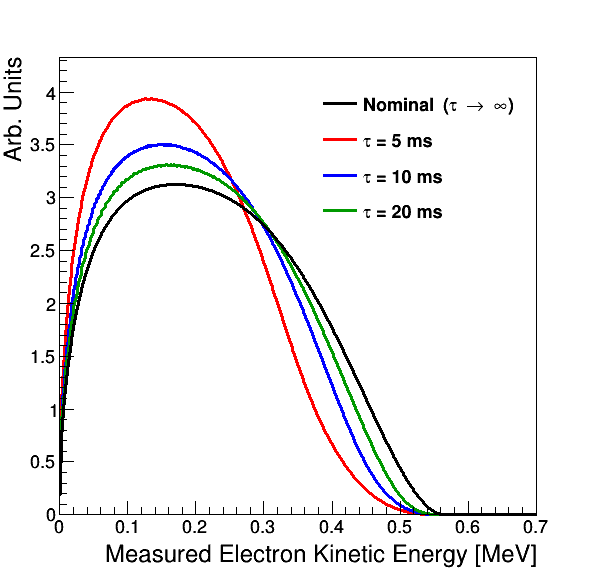
\includegraphics[width=.49\textwidth]{Ar39_energyPlot_DUNESPFD_lifetime.png}
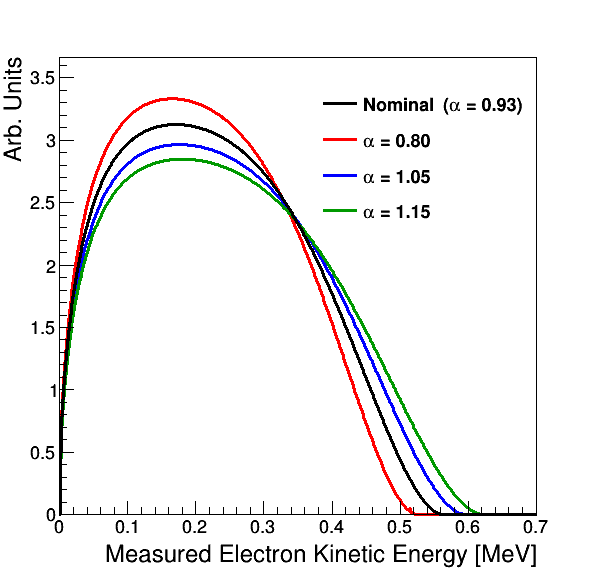
\includegraphics[width=.49\textwidth]{Ar39_energyPlot_DUNESPFD_recomb.png}
\end{dunefigure}

Using the fact that the ${}^{39}$Ar beta decays are uniformly distributed in the drift direction, one is able to precisely determine the expected reconstructed energy spectrum for a given set of detector response parameters. This can be done independently of using timing information (e.g.~from prompt scintillation light). As an example, one can use the reconstructed ${}^{39}$Ar beta decay energy spectrum to constrain primary detector response parameters such as the electron lifetime and recombination simultaneously. Figure~\ref{fig:ar39} illustrates the different possible reconstructed ${}^{39}$Ar beta decay electron energy spectra one might see after correcting for all other detector effects except for electron lifetime, for ${}^{39}$Ar beta decays occurring in the \dword{spmod}. Also shown in Figure~\ref{fig:ar39} is the impact of varying the true recombination model from the one assumed in energy reconstruction of the ${}^{39}$Ar beta decay electron, with infinite electron lifetime. The impact on the reconstructed energy spectrum is very different for the two detector effects, allowing for simultaneous determination of both quantities.

\subsubsection{Limitations}
%Strongly threshold driven, or noise issues. Translated to MeV limit. What is it? How does it change under noise assumptions? Before call it a big option, confirm noise issues. Is it disastrous?
There are several factors that impact the observed charge spectrum from ${}^{39}$Ar beta decays such as electronics noise, electron lifetime and recombination fluctuations. The effect of electron lifetime is more pronounced in dual phase due to the longer drift distance requiring the measurement be carried out more precisely. Also for this method to work, noise level must not be too high (requires less than \num{1000} e$^{-}$\,ENC) and a precision noise measurement is required. Another limitation of this method is that ${}^{39}$Ar beta decays closer to the cathode will be more likely to be below threshold (and thus undetected) in comparison to ones closer to the anode. This can impact the interpretation of the result. Extrapolating to regions closer to the cathode requires making the assumption that the electron lifetime is constant as a function of the drift coordinate, which may not be the case. In the case that there is variation in $x$, one could make use of an auxiliary measurement using $t_{0}$-tagged cosmic muon tracks to determine the dependence of electron lifetime on $x$.  However, this would require integrating over a much larger period of time in order to obtain the appropriate level of statistics.  External radiological sources may be able to make this measurement in limited parts of the detector more quickly, though this requires further study.

%it mainly probes regions closer to the anode; extrapolations to other regions in drift requires the electron lifetime be constant across the volume. One can use cosmic rays in these regions to mitigate this limitation, but a lower electron lifetime can complicate this process. 

%It should be mentioned that Ar39 beta decays closer to the cathode will be more likely to be below threshold (and thus undetected) in comparison to ones closer to the anode.  While this is folded into the electron lifetime measurement and so would not bias the result, it does impact the interpretation of the result; this is because the extracted electron lifetime would be more representative of regions of the detector closer to the anode.  Extrapolating this to regions closer to the cathode requires making the assumption that the electron lifetime is constant as a function of the drift coordinate, which may not be the case, though it is more likely to be uniform in the drift coordinate (total drift length of 3.6~m in $x$) than in the other two directions, along which the detector has greater extent (12~m in $y$, 58~m in $z$).  In the case that there is variation in $x$, one could make use of an auxiliary measurement using $t_{0}$-tagged cosmic muon tracks to determine the dependence of electron lifetime on $x$.  However, this would require integrating over a much larger period of time in order to obtain the appropriate level of statistics.  External radiological sources may be able to make this measurement in limited parts of the detector more quickly, though this requires further study.

One important consideration is whether or not the DUNE \fardet DAQ system can provide the necessary rate and type of data in order to successfully carry out this calibration at the desired frequency and level of spatial precision. From studies at \microboone, an estimate of the number of decays necessary to carry out a percent-level calibration of electron lifetime is $O(\mathrm{250k})$. 
%This means that in order to make a single measurement of electron lifetime in an entire DUNE far detector module, one would only need roughly five readout events (note $O(\mathrm{50k})$ decays per readout window per 10 kt module). 
However, one must also allow for the electron lifetime to spatially vary throughout the entire \SI{10}{\kt} module; it is not clear how much variation one should expect in a detector of this size. For a granularity of one measurement in every $\mathrm{m}^{2}$ drift volume once per day, a roughly 1~Hz for minimum-bias event trigger rate is needed; this is comparable to other \lartpc detectors that are currently operating. The data rate would be roughly \SI{4}{\giga\byte\per\s} for an entire \SI{10}{\kt} module without zero suppression. 
%A reasonable (though arbitrary) level of granularity to serve as a benchmark is one measurement per $\mathrm{m}^{2}$ (recall that the measurement is averaged over the drift direction, and thus is made in only two dimensions). Measurements with this level of granularity would require $O(\mathrm{100k})$ readout events (5~ms in length). This results in a requirement of roughly 1~Hz for minimum-bias event trigger rate in order to perform this calibration once per day, as is done at other LArTPC detectors that are currently operating. 

%The 1~Hz rate could either be obtained through hardware triggers issued at 1~Hz or hardware triggers issued at a higher rate and then pre-scaled in software. Minimum-bias triggers are sufficient as there are plenty of ${}^{39}$Ar beta decays in every event readout. Taking minimum-bias triggers at 1~Hz.

%This leads to a data rate of roughly 4~GB/s for an entire 10~kt module without zero suppression. With zero suppression, using a threshold based upon noise levels expected at the DUNE far detector (400-500 electrons for collection plane wires), one arrives at roughly 5~MB/s. The data rate for the zero-suppressed case takes into account the use of a three wire by 40~time tick window for each candidate decay in a single plane; this window was determined to be optimal for studies at MicroBooNE, and would only be tweaked slightly for DUNE. 

Note that the DAQ rates estimated previously do not take into account the need to save the required amount of data on the induction planes, which will have higher noise levels. It might be necessary to save data from many induction plane wires for a candidate ${}^{39}$Ar beta decay found on a single collection plane wire, leading to a much higher data rate (a factor of $O(100)$ higher). One can get around this requirement by making the electron lifetime measurement strictly in the $z$ direction (by far the longest dimension of the detector, and thus the most interesting to probe for spatial variations of electron lifetime), or by introducing a tighter requirement on the reconstructed charge threshold for the induction planes.

%%%%%%%%%%%%%%%%
\subsubsection{Remaining Studies}
Currently, the plan is to study this calibration technique in more detail first with data from \dword{protodune}, well in advance of first operations with the \dword{fd}, to %understand lessons learned and challenges for DUNE.
gain lessons learned and understand the challenges for DUNE.

%SG: don't want to include the following, extra stuff from MM:
%Characterizing the raw ${}^{39}$Ar  beta decay charge spectrum in a smaller device (capable of tagging light associated with individual ${}^{39}$Ar  beta decays in order to correct electron lifetime on a decay-by-decay basis) ahead of first operations of the DUNE far detector will increase the precision of the electron lifetime measurement at DUNE.  Such a device should be placed deep underground in order to ensure effectively zero contamination from charge or light of cosmogenic origin. 

%Notes from SG :Some specific studies that can help here are: 1. Simulation studies to understand the limitation in the usability of the source if we do not achieve the noise levels we want.  2. What is the dependence of electron lifetime on signal? Simulation studies to understand the impact of electron lifetime for DUNE. Can one take low purity and high purity data at \microboone and do this study? 3. Continue developing techniques to use this source for calibration studies at uB and \dword{protodune}. This will validate the analysis techniques and benchmarks what can be achieved from this source. 4. Take the techniques developed at uB/\dword{protodune} and understand what parameters/variables need to be tuned to extrapolate the techniques to DUNE and assess (with simulation studies) what impact those variables will have on the results. 5. Any \dword{daq} related studies to mitigate the issues with high rates?

%%%%%%%%%%%%%%%%%%%%%%%%%%%%%%%%
\subsection{Instrumentation and Monitoring Data }
\label{sec:inst}
%- written by Sowjanya}
Several instrumentation and detector monitoring devices %that 
will provide valuable information for calibrations. %In addition to instrumentation data, there will also be detector monitoring data that can provide useful information for calibrations and physics and also inform about the stability of various detector variables.
The cryogenics instrumentation and detector monitoring effort for DUNE is centrally led by the Cryogenics Instrumentation and Slow Controls (CISC) consortium. The %se 
instrumentation devices include liquid argon temperature monitors, \lar purity monitors, gaseous argon analyzers, and cryogenic (cold) and inspection (warm) cameras. %There are 
Other instrumentation devices such as drift \dword{hv} current monitors and external charge injection systems %that 
will be useful for calibrations that will be led by the High Voltage and TPC Cold Electronics consortia, respectively. The computational fluid dynamics (CFD) simulations play a key role for calibrations initially in the design of the cryogenics recirculation system, and later for %physics when the CFD simulations are validated using cryogenics instrumentation data. 
physics studies when the cryogenics instrumentation data is used to validate the simulations. This section provides a brief description of possible measurements with various instrumentation devices and %also what 
of the detector monitoring data that will be useful for calibrations.

%%%%%%%%%%%%%%%%
\subsubsection{Possible Measurements}
Electro-negative contaminants such as oxygen and water in the \lar can absorb signal electrons created from the ionization of argon atoms. The gas analyzers can be used for measuring these contaminants in the liquid. There is a plan to deploy a gas analyzer system for DUNE that will be capable of taking measurements at multiple points around the cryogenics system. In addition to gas analyzers, purity monitors provide quick measurements of \lar purity by measuring electron lifetime (%through
via the anode-to-cathode charge ratio) in a small space, typically less than a meter. The purity monitor measurements are especially useful during detector commissioning and initial operations when cosmic-ray data will not be available to perform more detailed studies. Electron lifetime correction is an important step in calorimetric reconstruction and can %also 
impact many other parameters such as electron recombination and track reconstruction. There is a plan to deploy three purity monitors inside the cryostat and some in the inline filters of the argon purification system. 

%There will be s
Several thermometers, both individual sensors and vertical temperature gradient monitors (both static and movable), %that 
will be installed throughout the volume of the cryostat %that will 
to provide \lar temperature measurements with a precision goal of \SI{5}{\milli\kelvin}. The biggest impact of \lar temperature is on the electron drift velocity through the drift coordinate, 
which in turn affects %detector 
the fiducial volume. Drift velocity can also impact measurements like electron diffusion. Both temperature and purity monitor data will be critical for validating the \lar flow model. Validation of the fluid-flow model using instrumentation data will give confidence %in using the model for projections for physics to understand impact of various liquid flow properties. 
in its projections regarding the impact of various liquid flow properties on the physics.
In addition to the instrumentation data, the cryogenics system data such as \lar contamination levels, temperatures and various flow parameters will be continuously monitored and recorded, providing additional information for calibrations.

DUNE plans to deploy both cryogenic cameras and inspection cameras. The cryogenic cameras will be used to look for \dword{hv} activity, especially breakdowns. The inspection cameras will be used to monitor the health of the detector components and to visually diagnose any issues that arise. % in case of issues. 
%Both of these data 
Data from both types of cameras will be useful for calibrations to understand any electric field anomalies or unexpected drift field responses. Additionally, to further monitor and diagnose \dword{hv} issues, installing devices such as current monitors will be useful to diagnose or characterize the \dword{fc}. The experience from \microboone using a source meter to continuously monitor pick-off point voltage with respect to the detector ground has helped the collaboration diagnose HV problems. In both SP and DP systems, the failure of a resistor will create a significant, local electric field distortion which will need to be identified. In the DP system, four registers would have to fail to cause a failure %of 
across the field cage gap, but even one failure in the SP can have an impact; this may be partially mitigated by modifying the HV.
% To be precise, the field distortion for the given gap would follow the formula is simply: V_bad-gap/V_normal-gap = R_bad-gap/R_normal-gap;  Where R_normal-gap=R_resistor*N_resistors-gap;  R_bad-gap=R_resistor*N_resistor-live-gap
%So if one resistor in one of the gaps die, we will see the field of this particular gap increased by 4/3=1.333

%%%%%%%%%%%%%%%%
\subsubsection{Limitations}
While purity monitors have practical advantages in terms of speed of measurement and the ability to measure low electron lifetimes before tracks can be reconstructed, purity monitor measurements are very localized and do not necessarily reflect any purity variations in the cryostat. Also, purity monitors typically measure the effect of the contaminants at a lower electric field. In fields above about \SI{200}{\V\per\cm}, the drift field increases the speed of the drift electrons 
\fixme{increases in the field cause increases in drift speed? pls clarify}
and this can lead to a different electron-capture cross section on the contaminants for the purity monitor and the drift electrons in the TPC. Additionally, purity monitors %also 
have a limited lifetime, making it important to be aware that %the measurements from them will not be available 
they will not be able to provide measurements for the entire lifetime of the experiment.
To mitigate this, \microboone has developed a nearline purity monitoring system that uses a statistically sufficient sample to make a purity measurement once every few hours using cosmic-ray muons. Developing similar techniques for DUNE will be very useful. The low cosmic-ray rate might be an issue for DUNE, but %one may be able 
it may be possible to make less frequent nearline measurements. 

The fluid flow within DUNE is a unique challenge and the fluid flow model needs validation. The fluid recirculates on the timescale of 21 days\todo{Need to confirm this number}, but 
there may be fluid exchanges %of fluid from the top and bottom of the detector SG:confirm
on shorter timescales. The liquid argon flow pattern, if steady state can trap some ions indefinitely causing stable eddies that can significantly impact the space charge distribution. \fixme{previous sentence needs work; I cannot parse it}
In \microboone the flow pattern is turbulent so this does not occur, but this is not understood yet for DUNE.
Temperature monitor data are used to validate the fluid flow model, but achieving the %needed measurement 
required precision with thermometers is a challenge. %which 
The precision will %can impact how well one can 
affect the quality of the fluid flow model validation.

The presence of a \dword{fc} resistor failure will be detectable, however it will not be possible to determine where it has failed spatially from monitoring data. The position must be determined by existing or in-situ calibration systems. 

%In the case of temperature monitors, achieving the needed precision is a challenge and will impact how well one can validate the fluid flow model using temperature data. 

%%%%%%%%%%%%%%%%
\subsubsection{Remaining Studies}
The remaining studies %one can do 
prior to the  TDR are: % the following:
\begin{itemize}
\item Validation of the fluid flow model using instrumentation data at \dword{protodune}. %will be very informative and valuable for DUNE. 
\item Implemention of a nearline purity monitoring using cosmic rays (as does \microboone) to understand the challenges of implementing such a system in a larger-scale detector.
\item Use of current CFD simulations to understand the range of variation for various flow-related parameters (e.g., overall temperature variation in the cryostat, overall impurity variation across the \detmodule) and propagation of those variations to calibration %and 
to understand the impact on physics.
\item CFD studies to understand how \lar flow can impact space charge and ion accumulation (both positive and negative ions). This will be especially critical for the \dword{dpmod} design due to the liquid-gas interface, as described in detail in Section~\ref{sec:DP}.
\end{itemize}
